\documentclass[12pt]{article}

\usepackage[english]{babel}
\usepackage[utf8x]{inputenc}
\usepackage{amsmath,amssymb}
\usepackage{graphicx}
\usepackage{tikz}
\usepackage{pgfplots}


\usetikzlibrary{shapes,decorations}
\usepackage{verbatim}

% NEEDED #1
\usetikzlibrary{arrows}
% For every picture that defines or uses external nodes, you'll have to
% apply the 'remember picture' style. To avoid some typing, we'll apply
% the style to all pictures.
\tikzstyle{every picture}+=[remember picture]
% By default all math in TikZ nodes are set in inline mode. Change this to
% displaystyle so that we don't get small fractions.
\everymath{\displaystyle}


\title{Learning Ti$k$Z for Cellular Biophysics and Modeling Figures}
\author{Gregory D.\ Smith}

\begin{document}
\maketitle

%\begin{abstract}
%Your abstract.
%\end{abstract}

\newpage

\section{My Ti$k$Z Examples}


\begin{figure}[h!]
\tikzstyle{mybox} = [draw=blue, fill=blue!10, very thick,
    rectangle, rounded corners,inner sep=5pt]
\tikzstyle{fancytitle} =[fill=blue, text=white, ellipse]
\begin{center}
\begin{tikzpicture}
\node [mybox] (boxanalytical) { 
\begin{tikzpicture}
\node[text width=6cm] {
\begin{eqnarray}
f(x) &=& 3x-x^2  \nonumber\\
f^\prime(x) &=&   3-2x  \nonumber\\[\baselineskip]
f^\prime(\bar{x}) &=&  3-2\bar{x} = 0  \nonumber\\
\bar{x} &=& \frac{3}{2} = 1\frac{1}{2}  \nonumber
\end{eqnarray}
\[
 f\left(\bar{x}\right) = 3\left( \frac{3}{2} \right)  - \left( \frac{3}{2} \right)^2
= \frac{9}{4}  = 2 \frac{1}{4} 
\]
};
\end{tikzpicture}

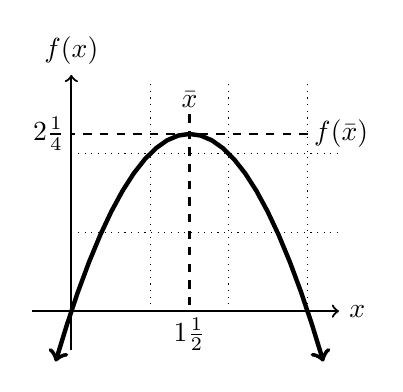
\begin{tikzpicture}
\draw[style=dotted] (0,0) grid (3.4,2.9);
\draw[ultra thick, domain=-0.2:3.2,<->] plot (\x, {-\x*\x +3*\x});
\draw[thick,->] (-0.5,0) -- (3.4,0) node[right] {$x$};
\draw[thick,->] (0,-0.5) -- (0,3.0) node[above] {$f(x)$};
\draw[thick,dashed] (1.5,2.5) node[above,inner sep=2pt] {$\bar{x}$} -- (1.5,0) node[below,inner sep=2pt] {$1\frac{1}{2}$};
\draw[thick,dashed] (3.0,2.25) node[right,inner sep=2pt] {$f(\bar{x})$} -- (0,2.25) node[left,inner sep=2pt] {$2\frac{1}{4}$};
 \end{tikzpicture}
 };
\node[fancytitle] at (boxanalytical.north) {Analytical / Pencil \& Paper}; 
\node[mybox,below=0.7cm] at (boxanalytical.south) (boxnumerical)  {
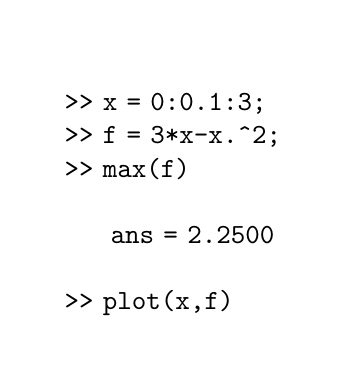
\begin{tikzpicture}[inner sep=10pt]
       \node[text width=3cm] {
   \begin{verbatim}
 >> x = 0:0.1:3;
 >> f = 3*x-x.^2;
 >> max(f)
        
      ans = 2.2500
 
 >> plot(x,f)
\end{verbatim}
};
\end{tikzpicture}
    
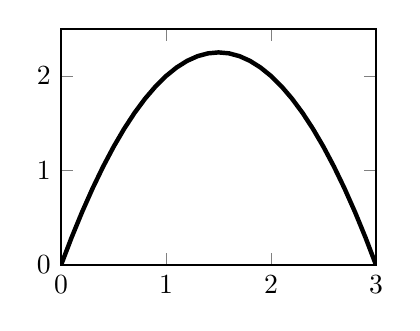
\begin{tikzpicture}
\begin{axis}[
width=4cm,
height=3cm,
scale only axis,
thick,
xmin=0,
xmax=3,
ymin=0,
ymax=2.5
]
\addplot [
color=black,
solid,
ultra thick,
forget plot
]
table[row sep=crcr]{
0 0\\
0.1 0.29\\
0.2 0.56\\
0.3 0.81\\
0.4 1.04\\
0.5 1.25\\
0.6 1.44\\
0.7 1.61\\
0.8 1.76\\
0.9 1.89\\
1 2\\
1.1 2.09\\
1.2 2.16\\
1.3 2.21\\
1.4 2.24\\
1.5 2.25\\
1.6 2.24\\
1.7 2.21\\
1.8 2.16\\
1.9 2.09\\
2 2\\
2.1 1.89\\
2.2 1.76\\
2.3 1.61\\
2.4 1.44\\
2.5 1.25\\
2.6 1.04\\
2.7 0.81\\
2.8 0.56\\
2.9 0.289999999999999\\
3 0\\
};
\end{axis}
\end{tikzpicture}
};
\node[fancytitle] at (boxnumerical.north) {Numerical / Computer};   
\end{tikzpicture}
\end{center}
\caption{No caption.}
\end{figure}

\newpage

\begin{figure}[h!]
\begin{center}
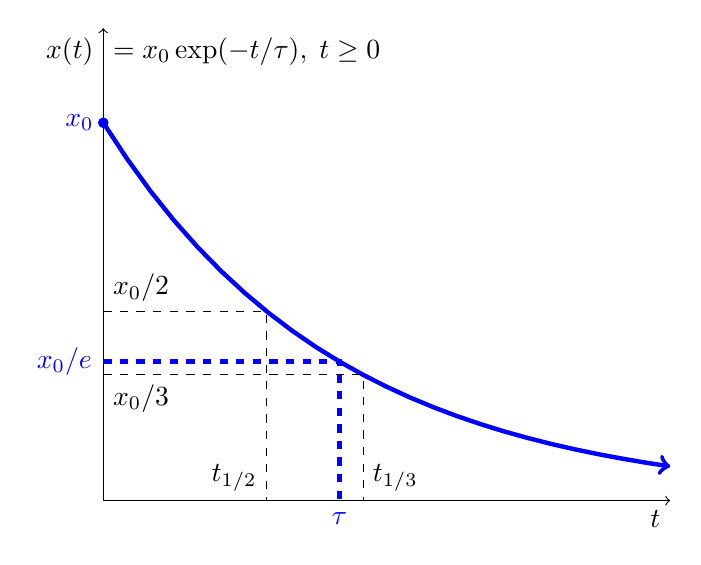
\begin{tikzpicture}[scale=0.6]
%\draw[help lines] (0,0) grid (10,10);
\draw[fill,blue] (0,8) circle [radius=0.1] node [left] {$x_0$};
\draw [<->]  (0,10) node [below left] {$x(t)$} node [below right] {$=x_0\exp(-t/\tau),\; t\geq 0$} -- (0,0) node [below left] {} -- (12,0) node [below left] {$t$};
       \draw[blue, ultra thick, domain=0:12] plot  (\x, {8*exp(-0.2*\x)}) [->];
\draw [ultra thick, dashed, blue]  (0,8/e) node [left] {$x_0/e$} -- (5,8/e) node [above right] {}
       -- (5,0) node [below] {$\tau$};
\draw [dashed]  (0,8/2) node [above right] {$x_0/2$} -- (5*0.69,8/2) 
       -- (5*0.69,0) node [above left] {$t_{1/2}$};
\draw [dashed]   (0,8/3) node [below right] {$x_0/3$} -- (5*1.1,8/3) 
       -- (5*1.1,0) node [above right] {$t_{1/3}$};
\end{tikzpicture}
\end{center}
\caption{The exponential decay $x(t)=x_0\exp(-t/\tau)$---equivalently, $x(t)=x_0e^{-t/\tau}$---evaluates to $x_0/e$ when $t=\tau$, that is, $x(\tau) =x_0 e^{-\tau/\tau} =x_0 e^{-1} =x_0/e$ where $e \approx 2.71$.  The exponential time constant $\tau$ is greater than $t_{1/2}$ (the half-time) and less than $t_{1/3}$ (the third-time, i.e., the time required for $x$ to decrease to $1/3$ its initial value). The initial value and exponential time constant are assumed to be positive: $x_0>0$, $\tau>0$.}
\end{figure}



\begin{figure}[h!]
\begin{center}
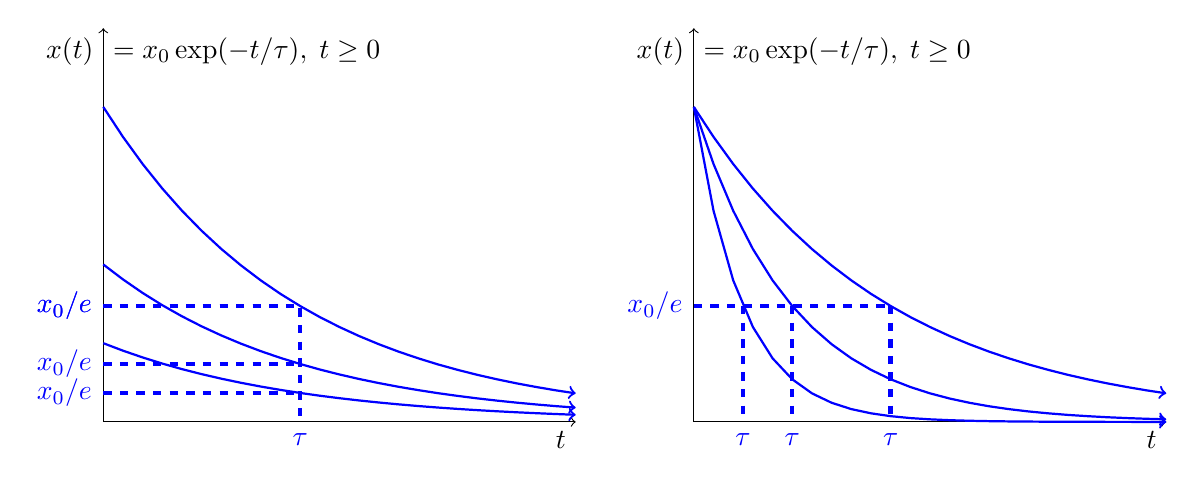
\begin{tikzpicture}[scale=0.5]
%\draw[help lines] (0,0) grid (10,10);
\draw [<->]  (0,10) node [below left] {$x(t)$} node [below right] {$=x_0\exp(-t/\tau),\; t\geq 0$} -- (0,0) node [below left] {} -- (12,0) node [below left] {$t$};
\foreach \y in {2,4,8} 
\draw[blue, thick, domain=0:12] plot (\x, {\y*exp(-0.2*\x)}) [->];
\foreach \y in {2,4,8} 
\draw [ultra thick, dashed, blue]  (0,\y/e) node [left] {$x_0/e$} -- (5,\y/e) node [above right] {};
\draw [ultra thick, dashed, blue]  (0,8/e) node [left] {$x_0/e$} -- (5,8/e) node [above right] {} -- (5,0) node [below] {$\tau$};
\draw [xshift=15cm,<->]  (0,10) node [below left] {$x(t)$} node [below right] {$=x_0\exp(-t/\tau),\; t\geq 0$} -- (0,0) node [below left] {} -- (12,0) node [below left] {$t$};
\foreach \y in {0.2,0.4,0.8} 
\draw[xshift=15cm,blue, thick, domain=0:12] plot (\x, {8*exp(-\y*\x)}) [->];
\draw [xshift=15cm,ultra thick, dashed, blue]  (0,8/e) node [left] {$x_0/e$} -- (1/0.2,8/e) node [above right] {};
%\draw[xshift=15cm,blue, thick, domain=0:12] plot (\x, {8*exp(-\y*\x)}) [->];
\foreach \y in {0.2,0.4,0.8}
\draw [xshift=15cm,ultra thick, dashed, blue](1/\y,8/e) node [above right] {} -- (1/\y,0) node [below] {$\tau$};
\end{tikzpicture}
\end{center}
\caption{XXXXThe exponential decay $x(t)=x_0\exp(-t/\tau)$---equivalently, $x(t)=x_0e^{-t/\tau}$---evaluates to $x_0/e$ when $t=\tau$, that is, $x(\tau) =x_0 e^{-\tau/\tau} =x_0 e^{-1} =x_0/e$ where $e \approx 2.71$.  The exponential time constant $\tau$ is greater than $t_{1/2}$ (the half-time) and less than $t_{1/3}$ (the third-time, i.e., the time required for $x$ to decrease to $1/3$ its initial value). The initial value and exponential time constant are assumed to be positive: $x_0>0$, $\tau>0$.}
\end{figure}





\section{Ti$k$Z Examples From Manual(s)}

\begin{figure}[h!]
\begin{center}
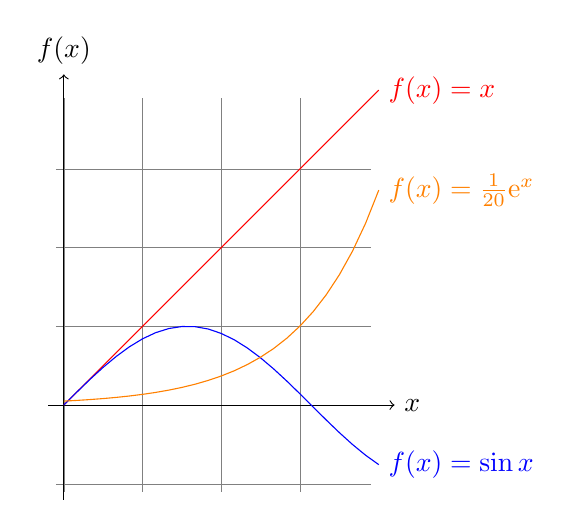
\begin{tikzpicture}[domain=0:4]
    \draw[very thin,color=gray] (-0.1,-1.1) grid (3.9,3.9);
    \draw[->] (-0.2,0) -- (4.2,0) node[right] {$x$};
    \draw[->] (0,-1.2) -- (0,4.2) node[above] {$f(x)$};
    \draw[color=red] plot(\x,{\x})
        node[right] {$f(x) =x$};
    \draw[color=blue] plot(\x,{sin(\x r)})
        node[right] {$f(x) = \sin x$};
    \draw[color=orange] plot(\x,{0.05*exp(\x)}) 
        node[right] {$f(x) = \frac{1}{20} \mathrm e^x$};
\end{tikzpicture}
\end{center}
\caption{Caption.}
\end{figure}


\begin{figure}[h!]
\begin{center}
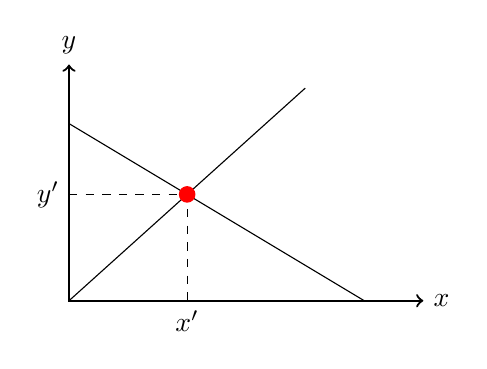
\begin{tikzpicture}[scale=1.5]
    % Draw axes
    \draw [<->,thick] (0,2) node (yaxis) [above] {$y$}
        |- (3,0) node (xaxis) [right] {$x$};
    % Draw two intersecting lines
    \draw (0,0) coordinate (a_1) -- (2,1.8) coordinate (a_2);
    \draw (0,1.5) coordinate (b_1) -- (2.5,0) coordinate (b_2);
    % Calculate the intersection of the lines a_1 -- a_2 and b_1 -- b_2
    % and store the coordinate in c.
    \coordinate (c) at (intersection of a_1--a_2 and b_1--b_2);
    % Draw lines indicating intersection with y and x axis. Here we use
    % the perpendicular coordinate system
    \draw[dashed] (yaxis |- c) node[left] {$y'$}
        -| (xaxis -| c) node[below] {$x'$};
    % Draw a dot to indicate intersection point
    \fill[red] (c) circle (2pt);
\end{tikzpicture}
\end{center}
\caption{Caption.}
\end{figure}


\begin{figure}[h!]
\begin{center}
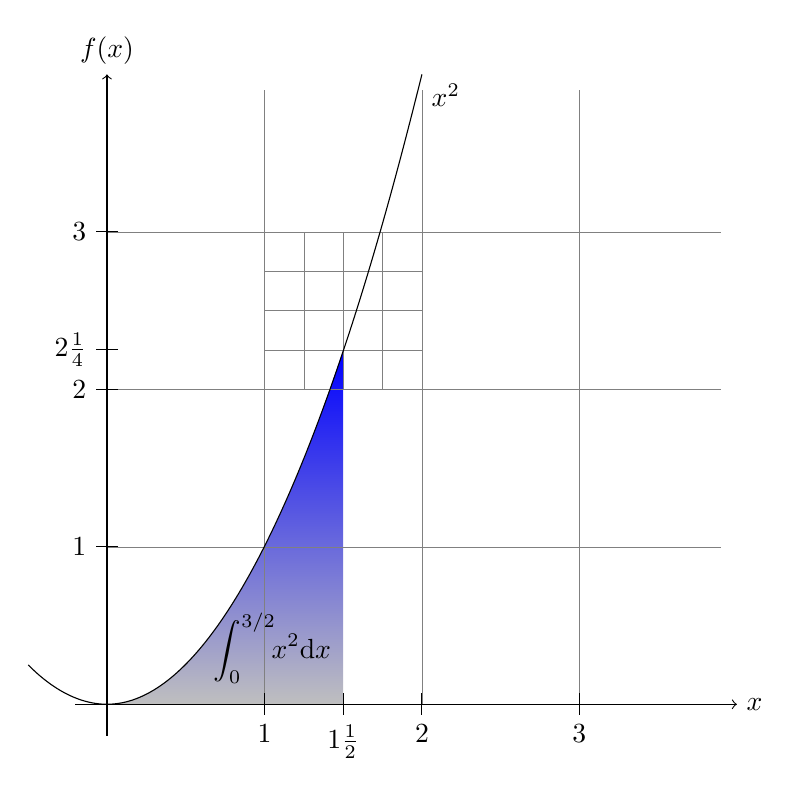
\begin{tikzpicture}[scale=2]
  \shade[top color=blue,bottom color=gray!50] 
      (0,0) parabola (1.5,2.25) |- (0,0);
  \draw (1.05cm,2pt) node[above] 
      {$\displaystyle\int_0^{3/2} \!\!x^2\mathrm{d}x$};

  \draw[style=help lines] (0,0) grid (3.9,3.9)
       [step=0.25cm]      (1,2) grid +(1,1);

  \draw[->] (-0.2,0) -- (4,0) node[right] {$x$};
  \draw[->] (0,-0.2) -- (0,4) node[above] {$f(x)$};

  \foreach \x/\xtext in {1/1, 1.5/1\frac{1}{2}, 2/2, 3/3}
    \draw[shift={(\x,0)}] (0pt,2pt) -- (0pt,-2pt) node[below] {$\xtext$};

  \foreach \y/\ytext in {1/1, 2/2, 2.25/2\frac{1}{4}, 3/3}
    \draw[shift={(0,\y)}] (2pt,0pt) -- (-2pt,0pt) node[left] {$\ytext$};

  \draw (-.5,.25) parabola bend (0,0) (2,4) node[below right] {$x^2$};
\end{tikzpicture}
\end{center}
\caption{Caption.}
\end{figure}


\newpage


% USES NEEDED #1

\begin{itemize}
    \item Coriolis acceleration
        \tikz\node [fill=blue!20,draw,circle] (n1) {};
\end{itemize}

% Below we mix an ordinary equation with TikZ nodes. Note that we have to
% adjust the baseline of the nodes to get proper alignment with the rest of
% the equation.
\begin{equation}
\vec{a}_p = \vec{a}_o+\frac{{}^bd^2}{dt^2}\vec{r} +
        \tikz[baseline]{
            \node[fill=blue!20,anchor=base] (t1)
            {$ 2\vec{\omega}_{ib}\times\frac{{}^bd}{dt}\vec{r}$};
        } +
        \tikz[baseline]{
            \node[fill=red!20,anchor=base] (t2)
            {$\vec{\alpha}_{ib}\times\vec{r}$};
        } +
        \tikz[baseline]{
            \node[fill=green!20,anchor=base] (t3)
            {$\vec{\omega}_{ib}\times(\vec{\omega}_{ib}\times\vec{r})$};
        }
\end{equation}

\begin{itemize}
    \item Transversal acceleration
        \tikz\node [fill=red!20,draw,circle] (n2) {};
    \item Centripetal acceleration
        \tikz\node [fill=green!20,draw,circle] (n3) {};
\end{itemize}

% Now it's time to draw some edges between the global nodes. Note that we
% have to apply the 'overlay' style.
\begin{tikzpicture}[overlay]
        \path[->] (n1) edge [bend left] (t1);
        \path[->] (n2) edge [bend right] (t2);
        \path[->] (n3) edge [out=0, in=-90] (t3);
 \end{tikzpicture}


\begin{figure}[h!]
\begin{center}
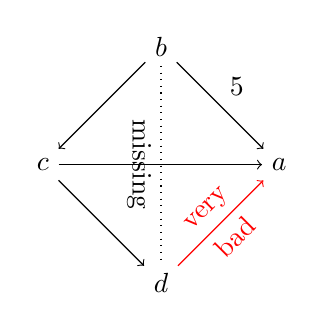
\begin{tikzpicture}
 \foreach \name/\angle in {a/0,b/90,c/180,d/270}
    \node (\name) at (\angle:1.5) {$\name$};
    \path[->] (b) edge            node[above right]  {$5$}     (a)
                  edge 	                                        (c)
                  edge [-,dotted] node[below,sloped] {missing} (d)
              (c) edge 	                                        (a)
                  edge 	                                        (d)
                  (d) edge [red]node[above,sloped] {very}
                  node[below,sloped] {bad}     (a); 
\end{tikzpicture}
\end{center}
\caption{aaaaaaa}
\end{figure}

\begin{figure}
\begin{center}
% Define box and box title style
\tikzstyle{mybox} = [draw=red, fill=blue!20, very thick,
    rectangle, rounded corners, inner sep=10pt, inner ysep=20pt]
\tikzstyle{fancytitle} =[fill=red, text=white]

\begin{tikzpicture}
\node [mybox] (box){%
    \begin{minipage}{0.50\textwidth}
        To calculate the horizontal position the kinematic differential
        equations are needed:
        \begin{align}
            \dot{n} &= u\cos\psi -v\sin\psi \\
            \dot{e} &= u\sin\psi + v\cos\psi
        \end{align}
        For small angles the following approximation can be used:
        \begin{align}
            \dot{n} &= u -v\delta_\psi \\
            \dot{e} &= u\delta_\psi + v
        \end{align}
    \end{minipage}
};
\node[fancytitle, right=10pt] at (box.north west) {A fancy title};
\node[fancytitle, rounded corners] at (box.east) {$\clubsuit$};
\end{tikzpicture}%
%
\tikzstyle{mybox} = [draw=blue, fill=green!20, very thick,
    rectangle, rounded corners, inner sep=10pt, inner ysep=20pt]
\tikzstyle{fancytitle} =[fill=blue, text=white, ellipse]
%
\begin{tikzpicture}[transform shape, rotate=10, baseline=-3.5cm]
\node [mybox] (box) {%
    \begin{minipage}[t!]{0.5\textwidth}
        Fermat's Last Theorem states that
        \[
            x^n + y^n = z^n
        \]
        has no non-zero integer solutions for $x$, $y$ and $z$ when $n > 2$.
    \end{minipage}
    };
\node[fancytitle] at (box.north) {Fermat's Last Theorem};
\end{tikzpicture}
\end{center}
\caption{kldfjadls;fjadl;sfj.}
\end{figure}


\begin{figure}[h!]
\center
\pgfmathsetseed{1}
\foreach \col in {black,red,green,blue}
{
  \begin{tikzpicture}[x=10pt,y=10pt,ultra thick,baseline,cap=round]
    \coordinate (current point) at (0,0);
    \coordinate (old velocity) at (0,0);
    \coordinate (new velocity) at (rand,rand);
    \foreach \i in {0,1,...,100}
    {
      \draw[\col!\i] (current point)
      .. controls ++([scale=-1]old velocity) and
                  ++(new velocity) .. ++(rand,rand)
         coordinate (current point);
      \coordinate (old velocity) at (new velocity);
      \coordinate (new velocity) at (rand,rand);
    }
  \end{tikzpicture}
}
\caption{This is the caption}
\end{figure}

\begin{figure}[h!]
\center

\begin{tikzpicture}
  \pgfsetfillopacity{0.5}
  \fill[red]   (90:1cm)  circle (11mm);
  \fill[green] (210:1cm) circle (11mm);
  \fill[blue]  (-30:1cm) circle (11mm);
\end{tikzpicture}
\caption{This is the caption}
\end{figure}

\begin{figure}[h!]
\center
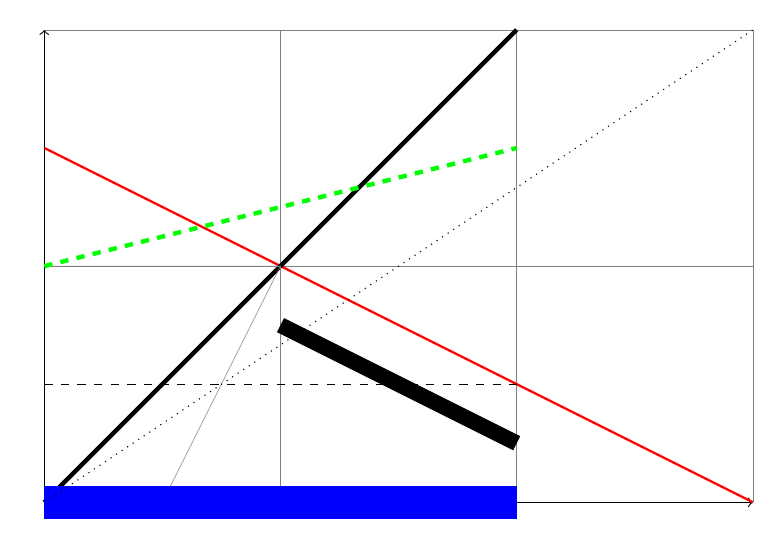
\begin{tikzpicture}[scale=3]
\draw[help lines] (0,0) grid (3,2);
\draw [<->] (0,2) -- (0,0) -- (3,0);
\draw [thick,red] (0,1.5) -- (3,0);
\draw [ultra thick] (0,0) -- (2,2);
\draw [help lines] (1,0) -- (1,1) -- (0,1);
\draw [help lines] (0.5,0) -- (1,1) -- (0,1);
\draw [line width=12,blue] (0,0) -- (2,0);
\draw [line width=0.2cm] (1,.75) -- (2,.25);
\draw [dashed, ultra thick,green] (0,1) -- (2,1.5);
\draw [dashed] (0, 0.5) -- (2,0.5);
\draw [dotted] (0,0) -- (3,2);
\end{tikzpicture}
\caption{This is the caption}
\end{figure}

\begin{figure}
\center
\begin{tikzpicture}[scale=4]
\draw [<->, rounded corners, thick, purple] (0,2) -- (0,0) -- (3,0);
\draw [blue] (0.5,0.5) rectangle (1.5,1);
\draw [red, ultra thick] (2,0.5) circle [radius=0.4];
\draw [green,thick] (2,2) arc [radius=0.5, start angle=45, end angle= 120];
\draw [red, ultra thick] (2,2) circle [radius=0.1];
\draw[very thick] (0.5,0.5) to [out=90,in=195] (2,1.5);
\end{tikzpicture}
\caption{}
\end{figure}


\begin{figure}
\center
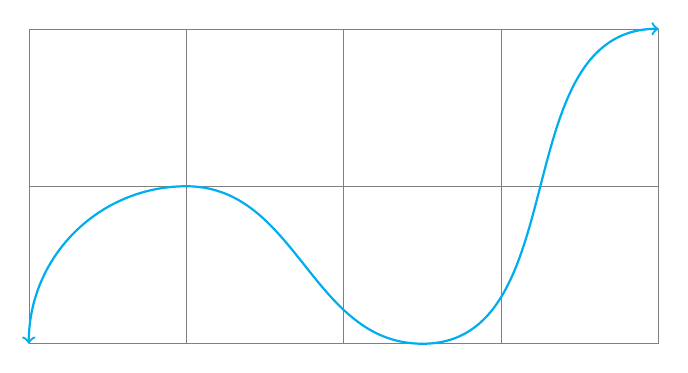
\begin{tikzpicture}[scale=2]
\draw[help lines] (0,0) grid (4,2);
\draw [<->,thick, cyan] (0,0) to [out=90,in=180] (1,1)
        to [out=0,in=180] (2.5,0) to [out=0,in=180] (4,2) ;
\end{tikzpicture}
\caption{}
\end{figure}

\begin{figure}
\center
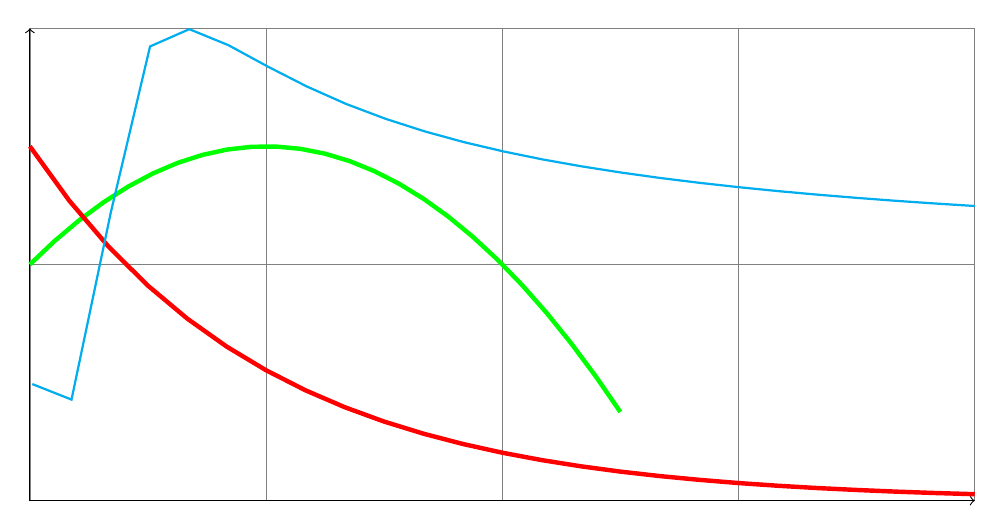
\begin{tikzpicture}[scale=3]
\draw[help lines] (0,0) grid (4,2);
\draw [<->] (0,2) -- (0,0) -- (4,0);
\draw[green, ultra thick, domain=0:2.5] plot (\x, {1+\x-0.5*\x*\x});
\draw[red, ultra thick, domain=0:4] plot (\x, {1.5*exp(-\x)});
\draw[cyan, thick, domain=0.01:4] plot (\x, {1+sin(pow(\x,-1) r)});
\end{tikzpicture}
\caption{}
\end{figure}

\begin{figure}
\center
\begin{tikzpicture}[scale=5]
\draw [thick, <->] (0,1) -- (0,0) -- (1,0);
\node [below right] at (1,0) {$x$};
\node [left] at (0,1) {$y$};
\draw [fill] (.4,.6) circle  [radius=.5pt];
\node [above right] at (.4,.6) {$A$};
\end{tikzpicture}
\caption{}
\end{figure}

\begin{figure}
\begin{center}
\begin{tikzpicture}
\draw[<->] (6,0) node[below]{$q$} -- (0,0) --
    (0,6) node[left]{$V(q)$};
\draw[very thick] (0,0) to [out=90,in=145] (5,4.5);
\end{tikzpicture}
\end{center}
\caption{}
\end{figure}


\begin{figure}
\begin{center}
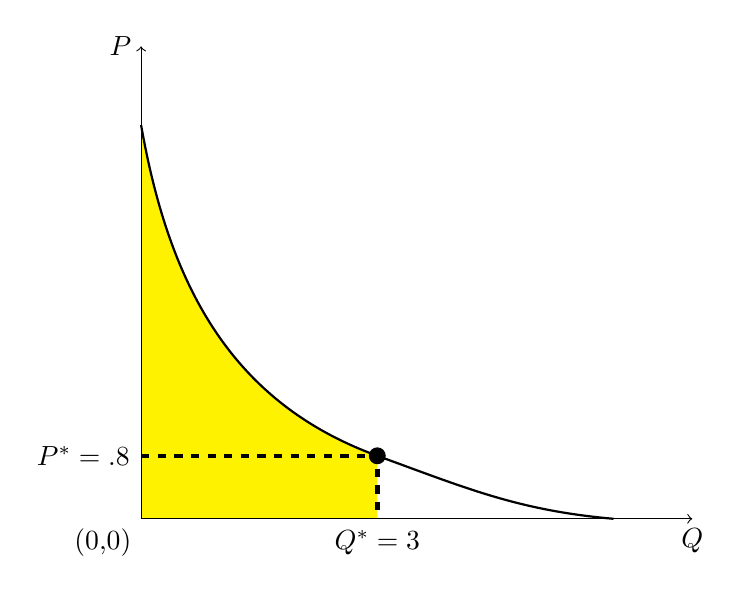
\begin{tikzpicture}
\path [fill=yellow] (0,0) -- (0,5) to [out=-80, in=160]
             (3,.8) -- (3,0) -- (0,0);
\draw [<->]  (0,6) node [left] {$P$}  -- (0,0)
       node [below left] {(0,0)} -- (7,0) node [below] {$Q$};
\draw [ultra thick, dashed]  (0,.8) node [left] {$P^*=.8$} -- (3,.8)
       -- (3,0) node [below] {$Q^*=3$};
\draw [fill] (3,.8) circle [radius=.1];
\draw [thick] (0,5) to [out=-80, in=160] (3,.8) to
             [out=-20, in=175] (6,0);
\end{tikzpicture}
\end{center}
\caption{}
\end{figure}



\end{document}